\documentclass[a4paper,12pt]{report}

\usepackage[utf8]{inputenc}     % Per caratteri accentati
\usepackage[T1]{fontenc}        % Font encoding
\usepackage[italian]{babel}     % Lingua italiana
\usepackage{lmodern}            % Font leggibile
\usepackage{geometry}           % Margini personalizzati
\geometry{margin=3cm}
\usepackage{setspace}           % Spaziatura
\onehalfspacing                 % Interlinea 1.5
\usepackage{graphicx}           % Immagini
\usepackage{float}              % Controllo posizionamento figure
\usepackage{amsmath, amssymb}   % Matematica
\usepackage{amsthm}             % Ambienti per teoremi, definizioni, ecc.
\usepackage{hyperref}           % Link ipertestuali
\usepackage{fancyhdr}           % Intestazioni e piè di pagina
\usepackage{titlesec}           % Formattazione titoli

% Definizione ambiente teorema numerato per capitolo
\newtheorem{theorem}{Teorema}[chapter]
\newtheorem{definition}{Definizione}[chapter]


\titleformat{\chapter}[display]
{\normalfont\huge\bfseries}
{}
{0pt}
{\Huge}

% Impostazioni intestazioni
\pagestyle{fancy}
\fancyhead{}
\fancyhead[LE,RO]{\thepage}
\fancyhead[RE]{\leftmark}
\fancyhead[LO]{\rightmark}

% Frontespizio personalizzabile
\begin{document}

    \begin{titlepage}
        \centering
        {\scshape\LARGE Università degli Studi di Milano \par}
        \vspace{1cm}
        {\scshape\Large Facoltà di Scienze e Tecnologie \par}
        \vspace{0.5cm}
        {\scshape\large Corso di Laurea in Informatica\par}
        \vspace{2cm}
        {\huge\bfseries Input Driven Pushdown Automata ed Edit Distances\par}
        \vspace{2cm}
        \begin{flushleft}
            \textbf{Relatore:} Giovanni Pighizzini\\
            \textbf{Candidato:} Luca Casnedi\\
            \textbf{Matricola:} 931856
        \end{flushleft}
        \vfill
        {\large Anno Accademico 2024--2025\par}
    \end{titlepage}

    \pagenumbering{Roman}
    \tableofcontents
    \clearpage

    \pagenumbering{arabic}

    \chapter{Introduzione}

    Gli \emph{Input Driven Pushdown Automata}, anche detti IDPDA, sono una classe di automi a pila in cui le operazioni sulla pila sono esclusivamente determinate dal simbolo di input. In particolare, il simbolo di input determina se l'automa compierà un'operazione di \emph{push} sulla pila, di \emph{pop}, oppure se lascerà la pila invariata.

    Gli IDPDA risultano particolarmente utili in diversi ambiti, tra cui il \emph{parsing} dei linguaggi di programmazione, dei documenti XML e, più in generale, in tutti i contesti in cui la struttura dell'input riflette la struttura gerarchica dei dati.

    È interessante notare come la famiglia dei linguaggi riconosciuti dagli IDPDA mantenga molte delle proprietà tipiche dei linguaggi regolari, pur essendo più ampia.

    Un problema di particolare rilevanza, dove gli IDPDA trovano utilizzo, consiste nel determinare la distanza tra una data stringa $s$ e un linguaggio $L$, detta anche \textit{distanza di edit}. Tale distanza è definita come il costo minimo di una sequenza di operazioni elementari di modifica su $s$ (sostituzione, inserimento, eliminazione di un simbolo), che la trasformano in una stringa $s' \in L$.

    In uno scenario applicativo, si può supporre di aver ricevuto in input una stringa appartenente a $L$, la quale potrebbe tuttavia contenere errori. L'obiettivo è quindi ricostruire, con la miglior accuratezza possibile, la stringa originaria.

    Per ottenere tale risultato, si può adottare un approccio a \emph{distanza minima}, ovvero determinare la stringa $y \in L$ tale che la \textit{distanza di edit} tra $x$ (la stringa ricevuta) e $y$ sia minima.

    \chapter{Definizioni}

    \section{Notazioni}
    
    Nel seguito, $\Sigma$ denota un alfabeto finito e $\Sigma^*$ è l'insieme delle stringhe su $\Sigma$, $\epsilon$ è la stringa vuota e la lunghezza di una stringa $w \in \Sigma^*$ è $|w|$. Dati gli insiemi $S$ e $T$, l'insieme delle funzioni parziali da $S$ a $T$ è denotato da $T^S$. La cardinalità di un insieme finito $S$ è $|S|$. Il simbolo $\perp$ denota la pila vuota e $2^S$ denota l'insieme delle parti dell'insieme $S$.

    \section{Input Driven Pushdown Automata}

    Una transizione di un IDPDA è determinata dal tipo di simbolo in input, appartenente all'alfabeto $\Sigma$, che stabilisce l'operazione da eseguire, eventualmente nulla.
    
    Si può rappresentare l'alfabeto di input di un IDPDA come unione di tre sottoinsiemi disgiunti e finiti:

    \begin{itemize}
        \item $\Sigma_{+1}$: parentesi sinistre, determinano una operazione di push sulla pila
        \item $\Sigma_{-1}$: parentesi destre, determinano una operazione di pop sulla pila
        \item $\Sigma_{0}$: simboli neutrali, non si traducono in operazioni sulla pila
    \end{itemize}

    Una stringa $s \in \Sigma$ è detta \textit{ben formata} se ogni parentesi sinistra ha una parentesi destra corrispondente, e viceversa.

    \section{Automi Input Driven Deterministici}

    \begin{definition}
        Un \textit{automa a pila input driven deterministico} (detto anche DIDPDA) è una settupla $A = (\Sigma, Q, \Gamma, q_0, \perp, \left[ \delta_a \right]_{a \in \Sigma}, F)$ dove:
        \begin{itemize}
            \item $\Sigma$ è un alfabeto di input, composto da tre sotto-insiemi finiti e disgiunti $\Sigma_{+1}$, $\Sigma_{-1}$, $\Sigma_{0}$
            \item $Q$ è l'insieme di stati dell'automa
            \item $q_{0} \in Q$ è lo stato iniziale
            \item $F \subseteq Q$ è il sottoinsieme degli stati \textit{accettanti}
            \item $\Gamma$ è  l'\textit{alfabeto della pila}
            \item $\perp$ è il simbolo che indica la pila vuota
            \item $\delta_{<} : Q \rightarrow Q \times \Gamma$ è la funzione di transizione che, per ogni parentesi sinistra $< \in \Sigma_{+1}$, dato un determinato stato corrente, fornisce lo stato successivo ed il simbolo da pushare sulla pila
            \item $\delta_{>} : Q \times (\Gamma\;\cup\perp) \rightarrow Q$ è la funzione di transizione che, per ogni parentesi destra $> \in \Sigma_{-1}$, dato un determinato stato corrente, fornisce lo stato successivo, posto che il simbolo specificato si trovi in cima alla pila e venga rimosso da essa o lo stack sia vuoto
            \item $\delta_{c} : Q \rightarrow Q$ è la funzione di transizione che, per ogni simbolo neutro $c \in \Sigma_{0}$, fornisce il prossimo stato
        \end{itemize}
    \end{definition}

    Data questa definizione del modello comportamentale di un DIDPDA alla lettura di un simbolo, si può subito notare come il contenuto della pila
    sia preso in considerazione solo quando il simbolo di input è una parentesi destra. 
    
    Quando il simbolo in input è, invece, un simbolo neutro o una parentesi sinistra, il prossimo stato non dipende dal contenuto dello stack.

    \clearpage
    \subsection{Esempio di DIDPDA}
    
    Per illustrare il funzionamento di un automa input driven deterministico, consideriamo il seguente esempio:
    
    \begin{figure}[H]
        \centering
        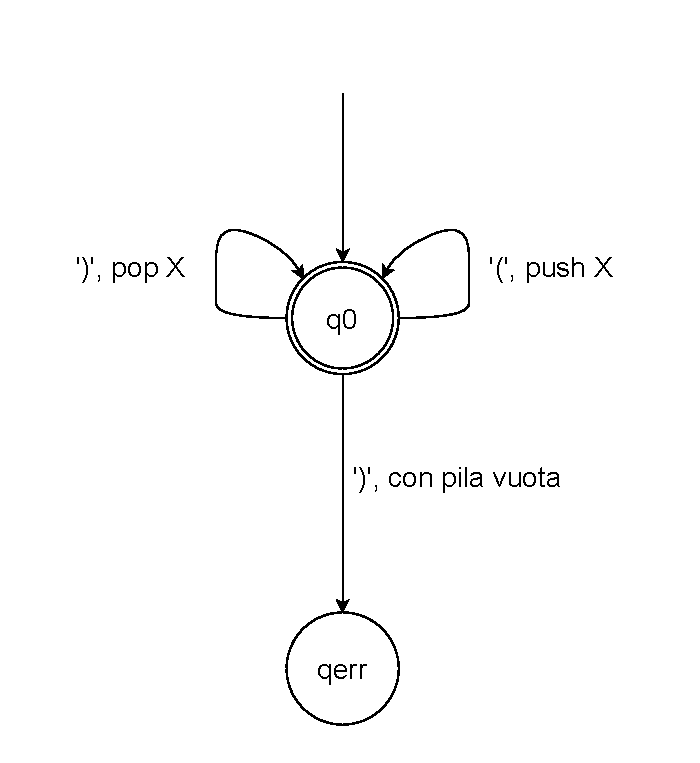
\includegraphics[width=4.2\textwidth,height=0.6\textheight,keepaspectratio]{img/automa_det}
        \caption{Esempio di automa input driven deterministico}
        \label{fig:esempio_didpda}
    \end{figure}

    Per l'automa rappresentato in Figura~\ref{fig:esempio_didpda}, gli alfabeti sono $\Sigma_{+1} = \{(\}$, $\Sigma_{-1} = \{)\}$, $\Sigma_0 = \emptyset$ e $\Gamma = \{X\}$.
    
    Le funzioni di transizione si possono definire come segue:

    \begin{align}
        \delta_{(}(q_0) &= \begin{cases}
        (q_0, X)
        \end{cases} \\[1em]
        \delta_{)}(q_0, \gamma) &= \begin{cases}
            q_0 & \text{se } \gamma = X \text{ (viene rimosso } X \text{ dalla pila)} \\
            q_{\text{err}} & \text{se } \gamma = \perp \text{ (pila vuota)}
        \end{cases}
    \end{align}

    In questo esempio non compaiono simboli neutrali.

    \section{Automi Input Driven non Deterministici}

    \begin{definition}
        Un \textit{non automa a pila input driven non deterministico} (detto anche NIDPDA) è una settupla $A = (\Sigma, Q, \Gamma, q_0, \perp, \delta, F)$ dove:
        \begin{itemize}
            \item $q_{0} \in Q$ è lo stato iniziale
            \item per ogni parentesi sinistra $< \in \Sigma_{+1}$, la funzione di transizione $\delta_{<} : Q \rightarrow 2^{Q \times \Gamma}$ fornisce, dato un certo stato attuale, un insieme di possibili risultati, ovvero coppie che indicano stato successivo e simbolo da caricare sullo stack
            \item per ogni parentesi destra $> \in \Sigma_{-1}$, la funzione di transizione $\delta_{>} : Q \times (\Gamma \cup \{\perp\}) \rightarrow 2^Q$, dato lo stato attuale e il simbolo in cima alla pila (che sarà rimosso se la pila non è vuota), fornisce un insieme di possibili stati successivi %lo stato successivo se viene effettuata una operazione di pop dallo stack del simbolo corrispondente
            \item per ogni simbolo neutro $c \in \Sigma_{0}$, c'è una funzione $\delta_{0} : Q \rightarrow 2^Q$
            \item l'alfabeto di input $\Sigma$, l'insieme degli stati $Q$, l'alfabeto della pila $\Gamma$, lo stack vuoto $\perp$ e l'insieme degli stati accepting $F \subseteq Q$ sono definiti come nella Definizione 2.1
        \end{itemize}
    \end{definition}

    Con gli automi non deterministici, la funzione di transizione è calcolata più volte per lo stesso input. 
    
    Una stringa è accettata se almeno una delle computazioni risultanti dalla lettura della stringa termina in uno stato \textit{accepting}.

    \section{Grammatiche Input-Driven}

    Gli Input Driven Pushdown Automata sono stati introdotti durante lo studio di particolari tipi di grammatiche, queste grammatiche sono definite
    con un alfabeto e una serie di regole che danno origine a stringhe che osservano vari criteri di \textit{corretta parentesizzazione}.
    
    Il primo dei modelli studiati sono state le \textit{grammatiche di parentesi} di McNaughton, nel quale l'alfabeto conteneva una parentesi sinistra $<$, una parentesi destra $>$
    ed una serie di simboli terminali, e le regole erano nella forma $X \rightarrow <\alpha>$, con $\alpha \in (\Sigma_0 \cup N)$ (dove $N$ è l'insieme dei simboli non terminali della grammatica), oppure nella forma $X \rightarrow c$ con $c \in \Sigma_0^*$.
    
    Tutte queste grammatiche vanno a dare origine a sottoclassi dei linguaggi input-driven.

    \begin{definition}
        Una grammatica input-driven è una quadrupla $G = (\Sigma, N, R, S)$ dove:
        \begin{itemize}
            \item $\Sigma = \Sigma_{-1} \cup \Sigma_0 \cup \Sigma_{+1}$ è l'alfabeto, diviso in tre sottoinsiemi disgiunti
            \item $N$ è l'insieme dei simboli non terminali
            \item $R$ è l'insieme delle regole, ognuna nella forma $A \rightarrow <B>C$, $A \rightarrow aC$, $A \rightarrow \epsilon$, dove $A, B, C \in N$, $< \in \Sigma_{+1}$, $> \in \Sigma_{-1}$, $a \in \Sigma$.
            \item $S$ è il simbolo iniziale
        \end{itemize}
    \end{definition}

    \section{Distanze di Edit}

    Il problema del calcolare le distanze di edit tra stringhe è strettamente correlato al problema del trovare la stringa con distanza di edit minima rispetto ad una data (correction problem).
    
    Una operazione di edit è una coppia $(a, b) \neq (\epsilon, \epsilon)$ con $\lvert a \rvert, \lvert b \rvert \leq 1$, ed è comunemente indicata con
    $a \rightarrow b$. 
    
    Una certa stringa $y$ può essere derivata da un'altra stringa $x$ tramite una operazione di edit $a \rightarrow b$, se $\exists v, w \in \Sigma^* \mid x = vaw, y = vbw$.
    
    Dati $a, b \in \Sigma, a \neq b$, possiamo definire le operazioni $a \rightarrow b$, $a \rightarrow \epsilon$ e $\epsilon \rightarrow a$ rispettivamente
    \textit{sostituzione}, \textit{cancellazione} e \textit{inserimento}.
    
    Ad ogni operazione di edit è associato un costo, rappresentato mediante la funzione $\gamma(a \rightarrow b)$.
    
    Data una sequenza di operazioni di edit $S = (s_1, s_2, ..., s_k)$, il costo di $S$ è definito come la somma dei costi delle singole operazioni di edit
    $\sum_{i=1}^{k} \gamma(s_i)$.

    Si assume che dati $x, y, k \in (\Sigma \cup \epsilon)$, $\gamma(x \rightarrow y) = 0$ se e solo se $x = y$, e $\gamma(x \rightarrow y)
    + \gamma(y \rightarrow k) \geq \gamma(x \rightarrow k)$.

    \begin{definition}
        Date due stringhe $x, y \in \Sigma^*$, la distanza di edit $d(x, y)$ da $x$ a $y$ è il minimo dei costi delle sequenze di operazioni di edit che trasformano $x$ in $y$.
    \end{definition}

    Questa definizione di distanza si può estendere, fissando un concetto di distanza che non riguarda due stringhe ma bensì una stringa e un linguaggio.
    
    \begin{definition}
        La distanza di edit tra un linguaggio $L \subseteq \Sigma^*$ ed una stringa $x \in \Sigma^*$ è il minimo tra i costi delle sequenze di operazioni di edit
        che trasformano stringhe di $L$ in $x$, ovvero $d(L, x) = min\{d(y, x) \mid y \in L \}$.
    \end{definition}


    \chapter{Sviluppo}

    Descrizione del lavoro svolto...

    \chapter{Risultati}

    Analisi e valutazione dei risultati...

    \chapter{Conclusioni}

    Osservazioni finali e possibili sviluppi futuri...

    \appendix
    \chapter{Appendice}

    Eventuali tabelle, codice o materiale integrativo...

    \clearpage
    \begin{thebibliography}{9}

        \bibitem{lamport}
        Leslie Lamport,
        \textit{LaTeX: A Document Preparation System},
        Addison Wesley, 1994.

% Aggiungere altre fonti

    \end{thebibliography}

\end{document}
